
\section{Introduction}
\label{sec:intro}

Low Power Wide Area Networks (LPWANs) are increasingly seen as an attractive
communication platform for city-scale Internet-of-Things (IoT) deployments.
They offer the ability to wirelessly connect energy-constrained devices to
gateways over distances of many kilometers. LPWANs also have power and cost
advantages over alternatives like cellular networks, particularly in
deploy-once, low maintenance and low throughput sensing applications.

While LPWANs are far from pervasive, the capabilities of networks like
LoRaWAN~\cite{Sornin2015, LoRaWanAlliance2015}, SigFox~\cite{centenaro2016}
and Ingenu's RPMA~\cite{Ingenu2015} have attracted investment and have spawned
early deployments. These technologies operate on the unlicensed ISM spectrum,
allowing businesses and consumers alike to deploy their own devices and
gateways. With Comcast’s recent announcement to integrate LPWAN radios into
future set-top boxes in the U.S.~\cite{comcast2}, LPWANs are likely
to grow rapidly. Given that each LPWAN gateway promises a range of up to ten
kilometers~\cite{LoRaWanAlliance2015}, major cities are likely to see a
fast-paced expansion in LPWAN coverage.

Despite the expected rise in density of LPWAN gateways, not all devices will
experience the promised 10 year battery life. Devices located in urban spaces
deep inside buildings or in remote neighborhoods will experience severe drain
in battery as their signals are highly attenuated even at the closest base
station. Some of these devices, such as those in basements or tunnels, may not
be in communication range of any gateway at all. Unlike cellular networks,
LPWANs are largely user-deployed and unplanned, meaning that these devices may
remain battery deprived or simply out of network reach in perpetuity, even as
thousands of gateways proliferate city-wide.

\begin{figure}[tb]
    \centering
    % \vspace{-10pt}
    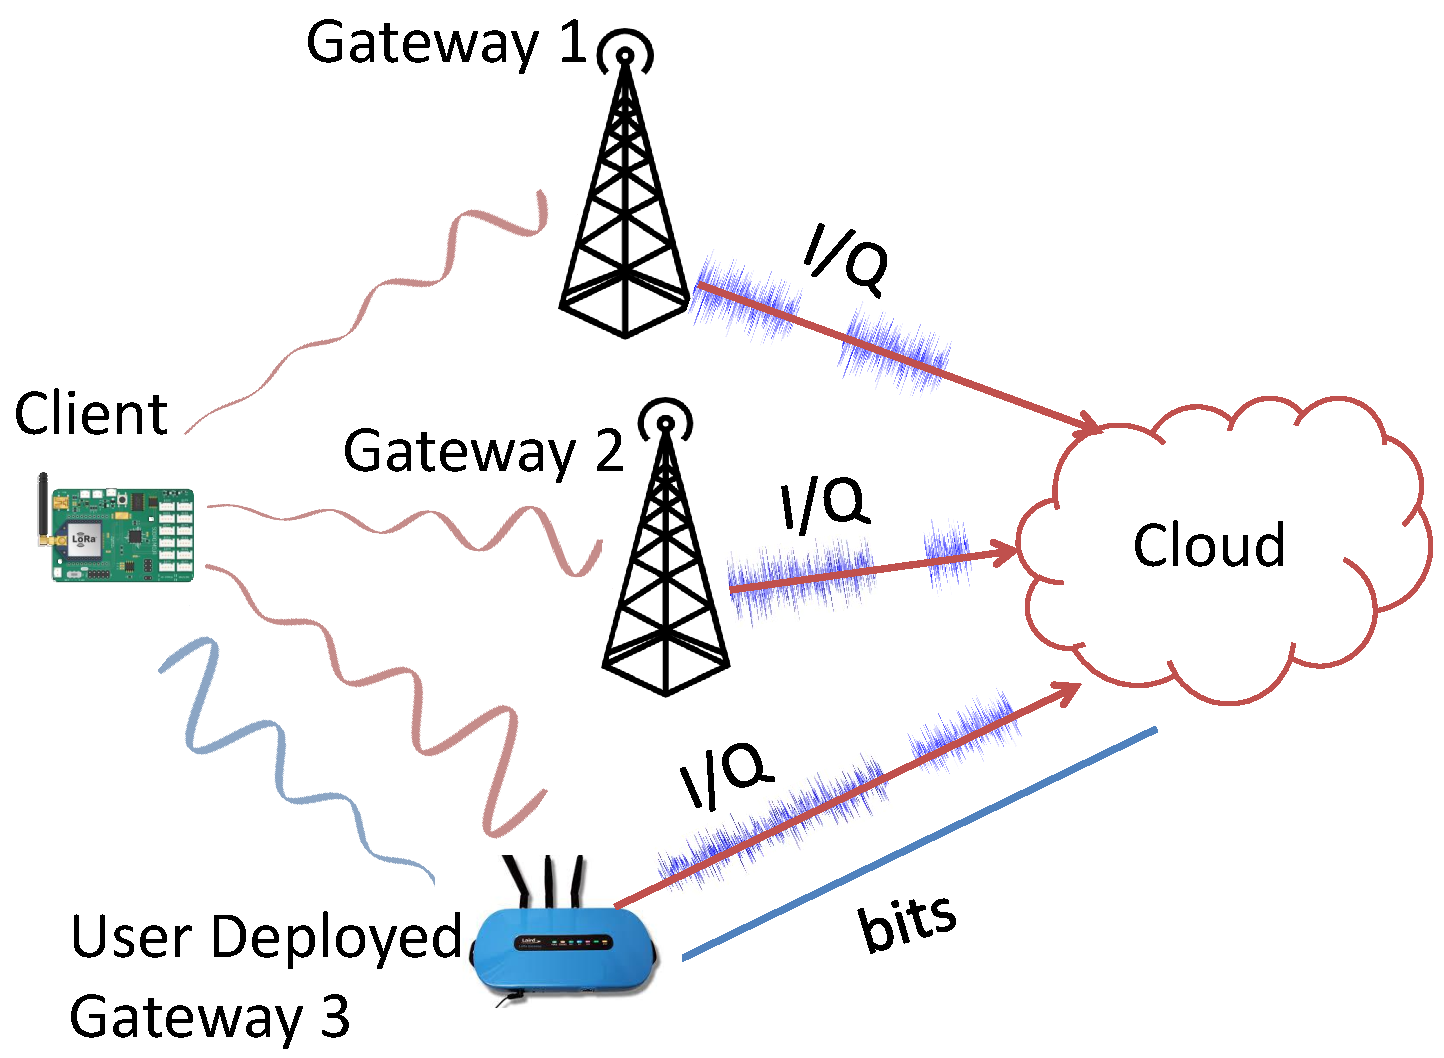
\includegraphics[width=0.60\columnwidth]{figures/LoRaRAN_cropped}
    \vspace*{-10 pt}
    \caption{Charm: LPWAN joint decoding in the cloud}
    \compactimg
    \label{fig:my_label}
\end{figure}

This paper presents Charm, a system that enhances the coverage of LPWANs and
the battery life of client devices in large urban deployments. Charm exploits
the observation that while signals from certain clients may attenuate
significantly, they are still likely to be received by multiple gateways in a
dense network. Charm introduces a hardware and software design at the gateways
that identifies and transports weak received signals to the cloud. We then
develop a joint decoding system at the cloud that coherently combines weak
signals received across multiple city gateways to decode the underlying data.
As a result, Charm both expands the decoding range of the LPWAN network and
improves battery-life for nodes already in range -- allowing client devices to
spend less energy per transmitted bit. Charm is built on the LoRaWAN
platform~\cite{LoRaWanAlliance2015}, a popular and widely available LPWAN
technology. Charm is implemented in a first-of-its-kind pilot deployment for
coherent diversity combining and demonstrates increased network coverage and
improved data rates across client devices.

While coherent diversity combining and PHY-layer processing in the cloud has
received much attention in the Wi-Fi~\cite{tan2009sam, xie2014scalable} and
cellular~\cite{checko2015cloud, wubben2014benefits} context, designing such a
system for low-power WANs offers radically new challenges. At the gateways, we
would have to decode very weak signals, weaker than 30 dB below the noise
floor. Simply uploading all received data to the cloud would overwhelm
the backend link, which is often  a simple home LAN. Both the LPWAN gateways
and clients are designed to be economical and deployed at scale, and without
the time synchronization required for coherent combining. At the cloud,
collating receptions from a large number of gateways at city-scale to identify
which of them contain packets from the same client is a challenge. We provide
an overview of our approach to address each of these challenges.

\noindent \textbf{Noise-Resilience at the Gateway:} The key challenge at the
gateway is identifying packets that are significantly below the noise floor
and, therefore, virtually undetectable. A straw-man approach to this problem
would be to correlate the received signal with a known preamble in any valid
packet. For instance, LoRaWAN uses a sequence of identical chirps -- signals
whose frequency increases linearly in time -- as a signature prefixing every
packet. In principle, sending an extremely long preamble could provide high
resilience to noise. In practice, doing so goes against the spirit of LPWANs
where energy for transmission is a valuable resource for the client.

Charm's approach to resolving this challenge is a hardware and software gateway
design that leverages the structure of the LoRaWAN LPWAN protocol.
Specifically, we develop a transform that converts the data symbols containing
\textit{a priori} unknown bits into a repeated and known sequence of signals,
much like the preamble. Charm can therefore now use both the preamble and the
modified data sequence to detect any packet.

To understand our approach at a high-level, we present an illustrative example
that dives into the details of the LoRaWAN PHY-layer. LoRaWAN transmits data
symbols as chirps whose initial frequency is a function of the data. For
instance over a bandwidth of 100 Hz, LoRa could represent the bit "0" as a
chirp starting at 2 Hz and bit "1" as a chirp starting at 52 Hz. Charm's
filter aliases the received LoRa signal so that frequencies modulo 50 Hz fold
into each other. This means that both bit "0" and bit "1" now map to an
identical chirp starting at 2 Hz. We apply this filter through the received
packet to obtain a repeated sequence of chirps as long as the entire packet
itself. This technique allows us to detect the packet with a much higher
resilience to noise compared to using the preamble alone, without incurring
additional overhead.

We develop a custom gateway hardware platform integrating a Semtech LoRaWAN
radio frontend, a low-power FPGA and Raspberry PI that can filter and detect
weak signals by processing received raw I/Q samples in real-time. Our hardware
platform, a hybrid between a full SDR and a dedicated high-performance radio,
is designed to be open and highly programmable -- a novel tool to experiment
with alternative LPWAN PHY-layer designs in the 900 MHz ISM band, without
compromising on signal quality or real-time performance.

\noindent \textbf{Scalability at the Cloud:} At the cloud, Charm must deal
with a large number of receptions from various gateways in a city, pruning for
weak signals and identifying common signals between gateways. Charm proposes
multiple optimizations to run its algorithms seamlessly at city-scale. For
instance, it is often the case that gateways transmit weak signals to the
cloud for packets that have already been decoded perfectly at other gateways.
However, realizing that the weak signal has already been decoded elsewhere is
impossible without decoding it in the cloud in the first place. Charm resolves
this chicken-or-egg dilemma by exploiting the timing and geographical location
of the received signal. Prior to sending any signal data to the cloud, a Charm
gateway sends the location, frequency, accurate timing and signal-to-noise
ratio (SNR) of the received weak packet. The cloud collates such information
across multiple gateways and requests for signals only from the gateways that
receive these signals the best. In doing so, Charm saves valuable uplink
bandwidth at the gateways and compution at the cloud. We describe how Charm
mitigates range of other important challenges at the cloud such as imperfect
timing, frequency offsets and overlapping transmissions.

We evaluate Charm in both indoor and outdoor environments using two testbeds
on the Carnegie Mellon University campus and around the city of Pittsburgh.
Eight user-deployed gateways built using our custom hardware platform support
a testbed covering a 0.6 sq.km. area around campus, which is used to study
Charm's performance with regard to local packet detection, range and
data-rates. Four rooftop gateways support the OpenChirp LPWAN network which
services a large 10 sq.km. area that we use to acquire traces for large-scale
simulations. Our results reveal the following:

\begin{itemize}
    \item {\bf Battery-Life: } By coherently combining across 8 base stations,
        Charm improves the SNR of a typical LoRaWAN transmission by 3.16 dB,
        extending battery life by up to 4$\times$.
    \item {\bf Range: } We improve the maximum communication range of 8 indoor
        user-deployed gateways in urban settings from 60m in LoRaWAN to 200
        meters using Charm, an overall increase in coverage area by
        10$\times$.
    \item {\bf Coverage: } Our trace-driven simulation, based on city-wide
        drive tests, estimates an overall increase in coverage by up to 2x due
        to Charm over LoRaWAN.
\end{itemize}

\noindent \textbf{Contributions:} We make the following novel contributions:
\begin{itemize}
    \item A technique that leverages the geographical diversity of unplanned,
        user-deployed gateways to enable joint decoding of weak transmissions.
        This improves battery-life for users in the network and increases the
        coverage area.
    \item A hardware platform and the underlying algorithms for detecting weak
        LoRaWAN transmissions locally at the gateway.
    \item A software architecture that builds atop of LoRaWAN to enable
        joint-decoding of signals in a scalable manner.
\end{itemize}